\chapter{Metodología}

Este capítulo describe el procedimiento seguido para el diseño y construcción del modelo experimental del túnel de viento a escala, así como la implementación de la lógica de adquisición y gestión de datos. Además, se detalla el desarrollo del modelo de simulación computacional (CFD) en ANSYS y la estrategia de validación que compara los resultados numéricos con los datos experimentales obtenidos. 

\section{Diseño y Construcción del Modelo Experimental}
\subsection{Estructura del Túnel de Viento a Escala}
El prototipo experimental se basa en un túnel de viento a escala que simula en forma generalizada un conducto de ventilación utilizados en minería subterránea. Se construyó una estructura cilíndrica suspendida en sus extremos mediante resortes. El material principal elegido fue acrílico transparente y plástico PLA debido a su resistencia, bajo peso y facilidad de perforación para montaje de dispositivos.

El túnel (Fig.~\ref{fig:cad_model} y Fig.~\ref{fig:explo}) presenta tres secciones principales:
\begin{enumerate}
    \item \textbf{Cámara de entrada:} Contiene un ventilador de computadora para generar el flujo de aire en el dispositivo.
    \item \textbf{Ducto principal:} Equipado con la instrumentación necesaria para la medición de variables operativas y la simulación de condiciones de ventilación minera.
    \item \textbf{Cámara de salida:} Contiene un ventilador adicional que opera como anemómetro calibrado para medir la velocidad del viento.
\end{enumerate}

Las dimensiones generales se muestran a continuación en la figura \ref{fig:sim}.

\begin{figure}[!ht]
    \centering
    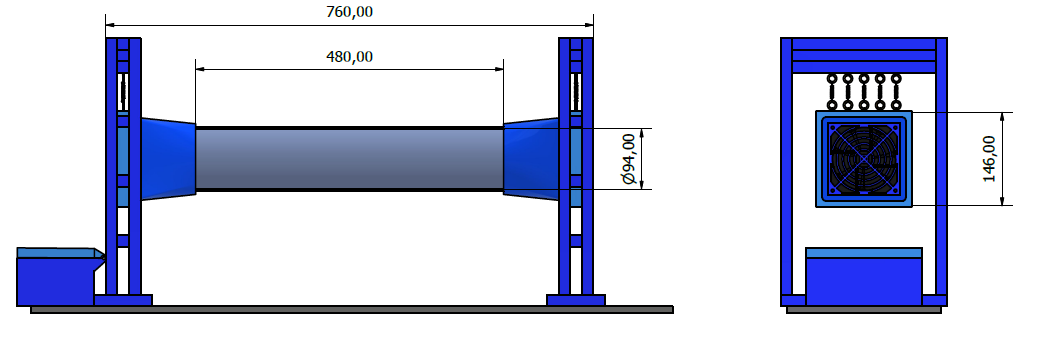
\includegraphics[width=0.8\linewidth]{images/dimen.png}
    \caption{Dimensiones generales del túnel de viento.}
    \label{fig:sim}
\end{figure}

\pagebreak

\begin{figure}[!ht]
    \centering
    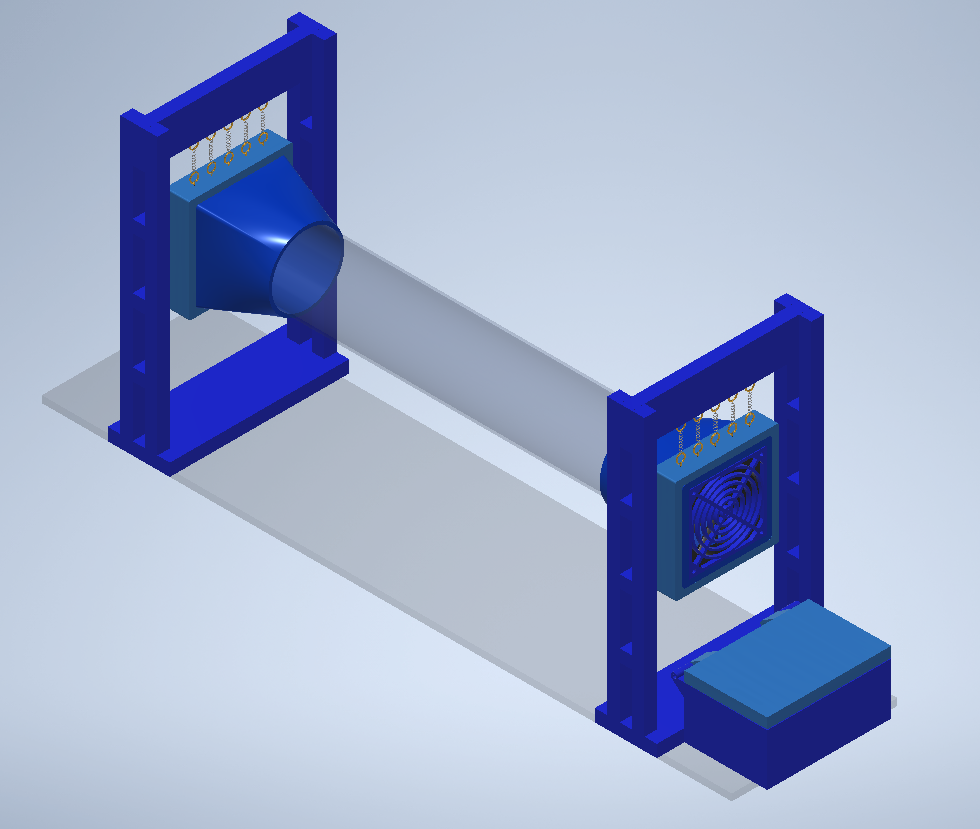
\includegraphics[width=0.5\linewidth]{images/exp.png}
    \caption{Vista isométrica del modelo CAD del dispositivo experimental.}
    \label{fig:cad_model}
\end{figure}

\begin{figure}[!ht]
    \centering
    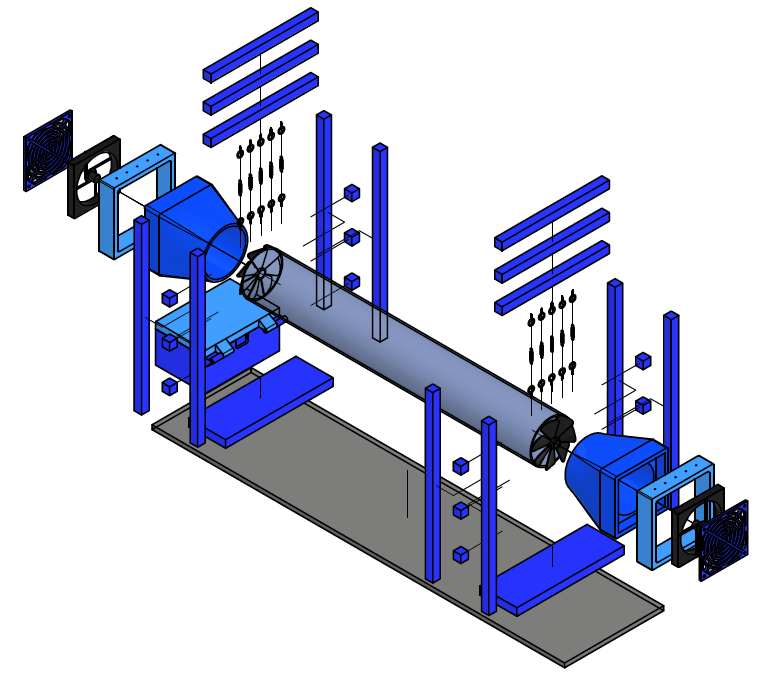
\includegraphics[width=0.5\linewidth]{images/explo.png}
    \caption{Vista explosionada del modelo CAD del dispositivo experimental.}
    \label{fig:explo}
\end{figure}

\subsection{Ventilador y Sistema de Control}
Se seleccionó un ventilador axial con capacidad de regular su velocidad mediante señal PWM. El ventilador, montado en la cámara de entrada, se sincroniza con el microcontrolador Arduino para variar las RPM (revoluciones por minuto) en función de los requerimientos del experimento y las pruebas de validación CFD. La transmisión de potencia y la robustez mecánica del montaje se verificaron para minimizar desbalances y vibraciones innecesarias.

\pagebreak
\section{Instrumentación y Disposición de Sensores}
\subsection{Sensores Seleccionados}
La selección de sensores descrita en el capítulo de Instrumentación respondió a la necesidad de medir variables eléctricas, mecánicas y térmicas. A continuación, se lista la disposición física de cada sensor en el túnel de viento:
\begin{itemize}
    \item \textbf{Sensor de Corriente ACS712:} Instalado en la línea de alimentación eléctrica del ventilador para medir el consumo de corriente.
    \item \textbf{Sensor de Voltaje PWM (0-25 V):} Conectado en paralelo al motor del ventilador para registrar la tensión aplicada y la modulación de ancho de pulso.
    \item \textbf{Sensor de Temperatura LM35:} Ubicado próximo al motor del ventilador para monitorear el sobrecalentamiento y la influencia de la velocidad de giro en la temperatura.
    \item \textbf{Cámara Térmica AMG8833:} Orientada hacia la carcasa del ventilador y las paredes del túnel para capturar un mapa térmico de la distribución del calor.
    \item \textbf{Acelerómetro MPU6050:} Montado en la base del ventilador para registrar vibraciones y movimientos provocados por desbalances en las aspas o resonancias del sistema.
    \item \textbf{Sensor de Flujo de Aire Indirecto (Anemómetro Calibrado):} Colocado dentro de la cámara de salida para medir la velocidad del flujo de aire.
\end{itemize}

La disposición de los sensores en el modelo experimental se detalla en la figura \ref{fig:sens}, y enumerados en la tabla \ref{tab:senso}.

\begin{figure}[!ht]
    \centering
    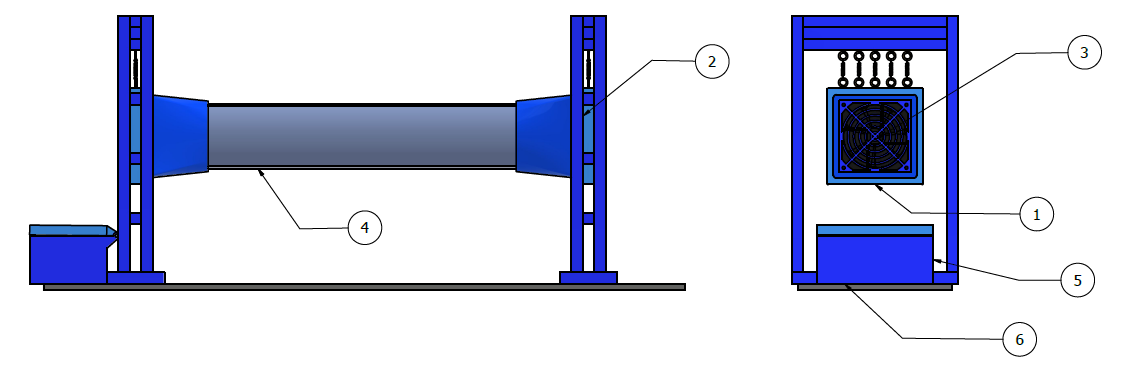
\includegraphics[width=0.8\linewidth]{images/sens.png}
    \caption{Esquema de disposición de los sensores.}
    \label{fig:sens}
\end{figure}

\begin{table}[H]
    \centering
    \caption{Listado de sensores utilizados.}
    \begin{tabular}{|c|l|l|}
    \hline
    \multicolumn{3}{|c|}{\textbf{Listado de sensores}} \\
    \hline
    \textbf{Elemento} & \textbf{Nombre}       & \textbf{Descripción}                          \\
    \hline
    1 & Acelerómetro      & Mide las vibraciones                       \\
    2 & Anemómetro        & Mide la velocidad de viento               \\
    3 & Termómetro        & Mide la temperatura del ventilador        \\
    4 & Cámara térmica    & Perfil de temperatura del ventilador      \\
    5 & Amperímetro       & Mide la corriente suministrada            \\
    6 & Voltímetro        & Mide el voltaje del ventilador            \\
    \hline
    \end{tabular}
    \label{tab:senso}
    \end{table}
    
\subsection{Integración con el Microcontrolador Arduino}
Todos los sensores se comunican con el microcontrolador Arduino a través de puertos analógicos o digitales, dependiendo de la naturaleza de la señal:
\begin{itemize}
    \item \textbf{ACS712 y Sensor de Voltaje PWM:} Conectados a las entradas analógicas para la lectura continua de la corriente y el voltaje.
    \item \textbf{LM35 y Anemómetro:} También acoplados a entradas analógicas; se utilizó un condensador de filtrado en el anemómetro para reducir el ruido.
    \item \textbf{MPU6050:} Comunicación digital I2C, que permite la transmisión simultánea de datos de acelerómetro y giroscopio.
    \item \textbf{AMG8833:} Comunicación digital I2C para la lectura matricial de valores de temperatura.
\end{itemize}

Se definieron tasas de muestreo específicas para cada sensor, equilibrando la precisión requerida con la capacidad de procesamiento. De esta manera, se evita la saturación en la transmisión de datos y se garantizan muestras representativas.

\section{Arquitectura de Adquisición y Procesamiento de Datos}
\subsection{Estructura General}
La lógica de adquisición y procesamiento de datos se compone de los siguientes elementos:
\begin{enumerate}
    \item \textbf{Microcontrolador Arduino:} Encargado de leer los sensores y controlar la velocidad del ventilador mediante señal PWM.
    \item \textbf{Servicio REST API:} Permite la interacción con la interfaz web y la base de datos, recibiendo peticiones para la configuración del ventilador o el inicio de la captura de datos.
    \item \textbf{Interfaz Web de Control:} Da acceso a los usuarios para ajustar la velocidad del ventilador, visualizar datos en tiempo real y seleccionar qué variables medir.
    \item \textbf{Base de Datos SQLite:} Se encarga de almacenar los datos de forma estructurada para su posterior análisis.
\end{enumerate}

\subsection{Programación del Sistema de Obtención de Datos}
En el microcontrolador Arduino se desarrolló un código modular, con las siguientes funciones principales:
\begin{itemize}
    \item \texttt{setup()}: Inicializa la comunicación con los sensores (I2C, puertos analógicos) y configura los pines de salida para la señal PWM.
    \item \texttt{loop()}: Ejecuta la rutina principal en la que se leen los valores de cada sensor, se calcula la media de las muestras durante un intervalo configurable y se envían los datos a través de la comunicación serial o Wi-Fi (dependiendo de la placa Arduino utilizada).
    \item \texttt{readSensors()}: Funciones individuales que retornan la lectura de corriente, voltaje, temperatura, vibración y flujo de aire.
    \item \texttt{setFanSpeed(value)}: Aplica la señal PWM para regular la velocidad de rotación del ventilador en función de un valor de consigna (0-255 en escalado Arduino o 0-100\%).
\end{itemize}

\section{Implementación de la REST API}
Para habilitar la comunicación entre Arduino y la aplicación web, se definió un servicio REST API (Representational State Transfer) ejecutado en una plataforma intermedia (por ejemplo, un servidor local o un \textit{single-board computer} con Linux). El servicio escucha peticiones HTTP (\texttt{GET}, \texttt{POST}) para:
\begin{itemize}
    \item \textbf{Configurar:} Cambiar la velocidad del ventilador o ajustar la frecuencia de muestreo de los sensores.
    \item \textbf{Iniciar/Detener la Lectura de Datos:} Gestionar los eventos de captura de información en el Arduino.
    \item \textbf{Obtener Datos:} Solicitar y recibir mediciones actualizadas en formato JSON, para ser almacenadas o visualizadas.
\end{itemize}

La conexión entre Arduino y este servicio puede realizarse de forma serial o inalámbrica (Wi-Fi o Bluetooth), dependiendo de la configuración elegida. El servicio REST API se programó en Python (utilizando el framework \texttt{Flask}), aunque pueden emplearse también entornos como Node.js o Java.

\section{Interfaz Web de Control y Selección de Datos}
\subsection{Diseño de la Interfaz}
La interfaz web (Fig.~\ref{fig:web}), accesible desde un navegador, proporciona una forma amigable de controlar el prototipo y visualizar la información en tiempo real. Sus secciones principales incluyen:
\begin{itemize}
    \item \textbf{Panel de Control de Velocidad:} Permite ajustar manualmente las RPM del ventilador o seleccionar modos automáticos predefinidos.
    \item \textbf{Panel de Datos en Tiempo Real:} Muestra gráficas de corriente, voltaje, temperatura, flujo de aire y vibración. Se utilizan librerías JavaScript como \texttt{Chart.js} o \texttt{D3.js} para la representación gráfica.
    \item \textbf{Selección de Variables a Medir:} El usuario define qué sensores deben estar activos y la frecuencia de muestreo para cada uno.
    \item \textbf{Historial de Lecturas:} Permite consultar y exportar datos pasados almacenados en la base de datos.
\end{itemize}

\begin{figure}[!ht]
    \centering
    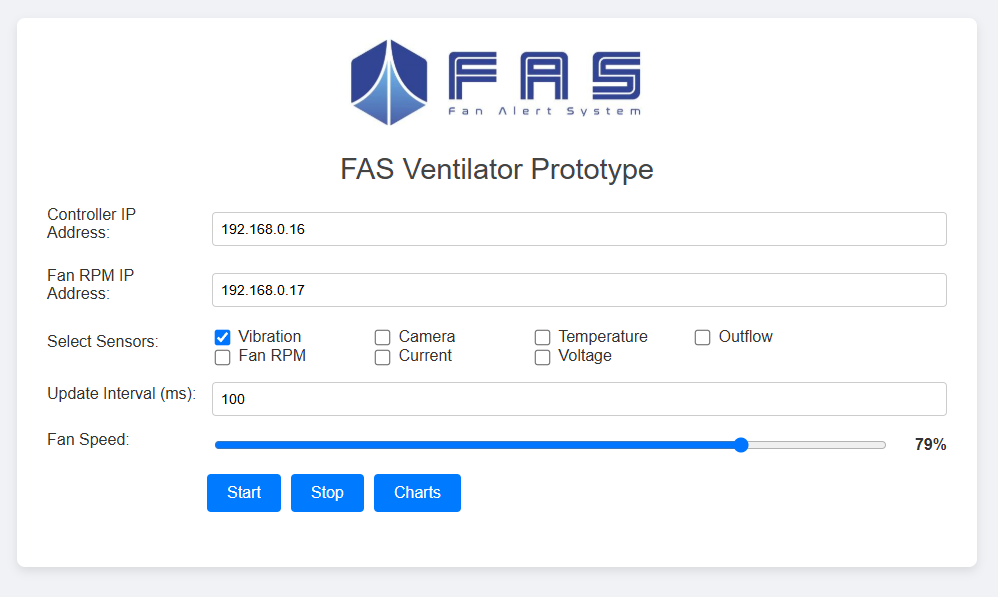
\includegraphics[width=0.8\linewidth]{images/web.png}
    \caption{Panel del control del dispositivo experimental.}
    \label{fig:web}
\end{figure}

\subsection{Interacción con la API}
La interfaz web se comunica con la API mediante peticiones \texttt{AJAX} (\texttt{GET} y \texttt{POST}), recibiendo datos en formato JSON. En cada consulta, el navegador interpreta la respuesta y actualiza dinámicamente la gráfica o los indicadores del panel de control.

\section{Almacenamiento de Datos en SQLite}
\subsection{Estructura de la Base de Datos}
Para el registro de la información se optó por SQLite, una base de datos liviana que no requiere un servidor dedicado, adecuada para prototipos y sistemas embebidos. La estructura contempla las siguientes tablas:

\begin{itemize}
    \item \texttt{measurements}: Almacena las lecturas de cada sensor. Los campos básicos incluyen:
    \begin{itemize}
        \item \texttt{id} (INTEGER, clave primaria autoincremental)
        \item \texttt{timestamp} (DATETIME)
        \item \texttt{sensor\_type} (TEXT) \textit{[p. ej. adxl345, amg8833, fanrpm, etc]}
        \item \texttt{value} (REAL)
    \end{itemize}
    
    \item \texttt{configurations}: Registra configuraciones de experimento, como la velocidad del ventilador, la frecuencia de muestreo y la duración de la captura.
    \begin{itemize}
        \item \texttt{id} (INTEGER, clave primaria autoincremental)
        \item \texttt{fan\_speed} (INTEGER)
        \item \texttt{sampling\_rate} (INTEGER)
        \item \texttt{date\_created} (DATETIME)
    \end{itemize}
\end{itemize}

\subsection{Inserción y Consulta de Datos}
Tras cada petición de lectura en el Arduino, la API recibe un paquete JSON con las mediciones, que posteriormente se insertan en la tabla \texttt{data}. Véase la figura~\ref{fig:table}.

\begin{figure}[!ht]
    \centering
    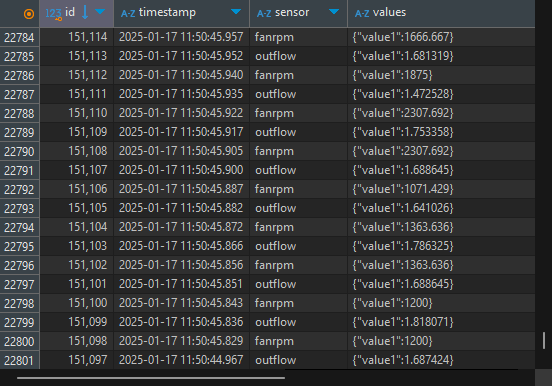
\includegraphics[width=0.5\linewidth]{images/table.png}
    \caption{Ejemplo de tabla de datos de sensores.}
    \label{fig:table}
\end{figure}

La consulta de datos se realiza directamente desde la base de datos, utilizando aplicaciones de gestión de base de datos para filtrar y exportar los datos según rangos de fechas, sensores y/o valores para su posterior análisis.

\newpage
\section{Simulación Computacional (CFD) en ANSYS}
\subsection{Preparación del Modelo CAD}
Para realizar la simulación CFD, se modeló la geometría del túnel de viento a escala en un software de diseño asistido por computadora (CAD). Se representó tanto la sección de entrada como la cámara principal, incluyendo la ubicación aproximada del ventilador. Este modelo 3D se exportó en un formato compatible (por ejemplo, \texttt{.igs} o \texttt{.step}) para ser importado posteriormente a ANSYS SpaceClaim (Fig.~\ref{fig:space}).

\begin{figure}[!ht]
    \centering
    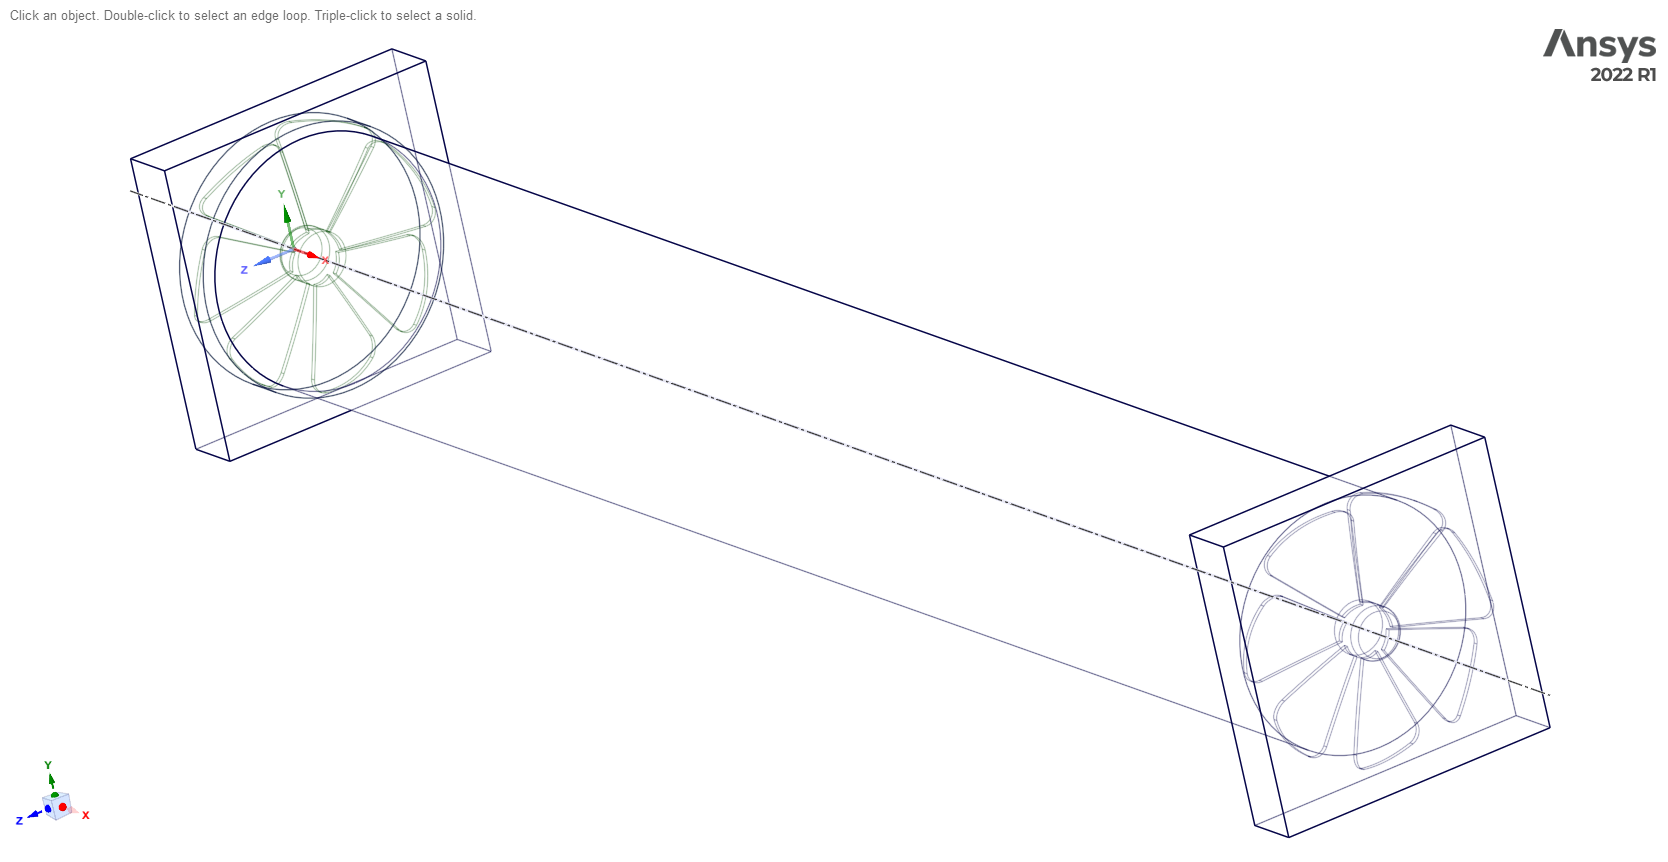
\includegraphics[width=0.8\linewidth]{images/space.png}
    \caption{Geometría del modelo en ANSYS SpaceClaim.}
    \label{fig:space}
\end{figure}

\newpage

\subsection{Configuración en ANSYS Fluent}
Una vez importada la geometría en ANSYS, se procedió a:
\begin{enumerate}
    \item \textbf{Creación de la malla:} Se generó una malla policéntrica compuesta por hexaedros y tetraedros, dependiendo de la complejidad de las cavidades. Se prestó especial atención a la región próxima al ventilador y a las zonas donde se esperaba mayor gradiente de velocidad. (Fig.~\ref{fig:mesh})
    \item \textbf{Selección del modelo de turbulencia:} Se optó por el modelo \texttt{k-$\epsilon$} estándar, apropiado para flujos internos con niveles moderados de turbulencia. 
    \item \textbf{Condiciones de contorno:} Se definió la entrada y salida de aire como una condición de velocidad o caudal (dependiendo del escenario). Se establecieron superficies sólidas con la pared del túnel y la carcasa del ventilador. (El flujo de aire se da por la diferencia de presión generada por la rotación del ventilador). En la figura \ref{fig:borde} se pueden apreciar las condiciones de contorno de manera gráfica. En azul la entrada de aire, en rojo la salida de aire y en amarillo la interfaz de la zona de rotación del ventilador.
    \item \textbf{Propiedades del fluido:} Se consideró aire como fluido ideal, con densidad aproximada de 1.225 kg/m$^3$ y viscosidad de $1.8 \times 10^{-5}$ Pa·s, a temperatura ambiente.
    \item \textbf{Configuración de la rotación del ventilador:} Para simular el efecto del ventilador, se definió una zona de rotación (\textit{rotating domain}) a una velocidad de rotación configurable según los experimentos.
\end{enumerate}

\begin{figure}[!ht]
    \centering
    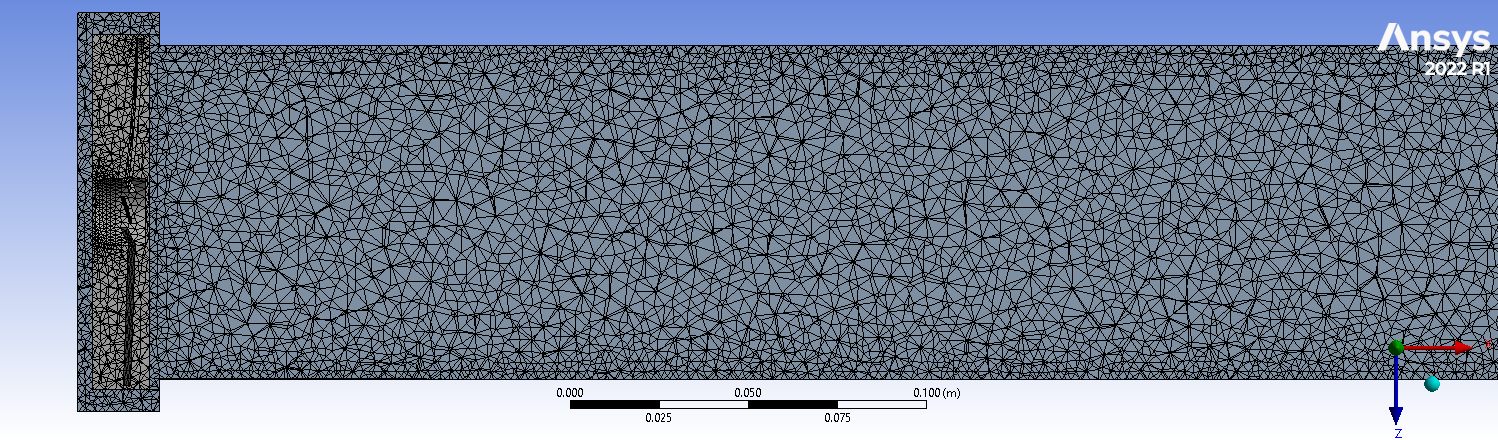
\includegraphics[width=0.7\linewidth]{images/mesh.png}
    \caption{Mallado realizado en ANSYS.}
    \label{fig:mesh}
\end{figure}

\begin{figure}[!ht]
    \centering
    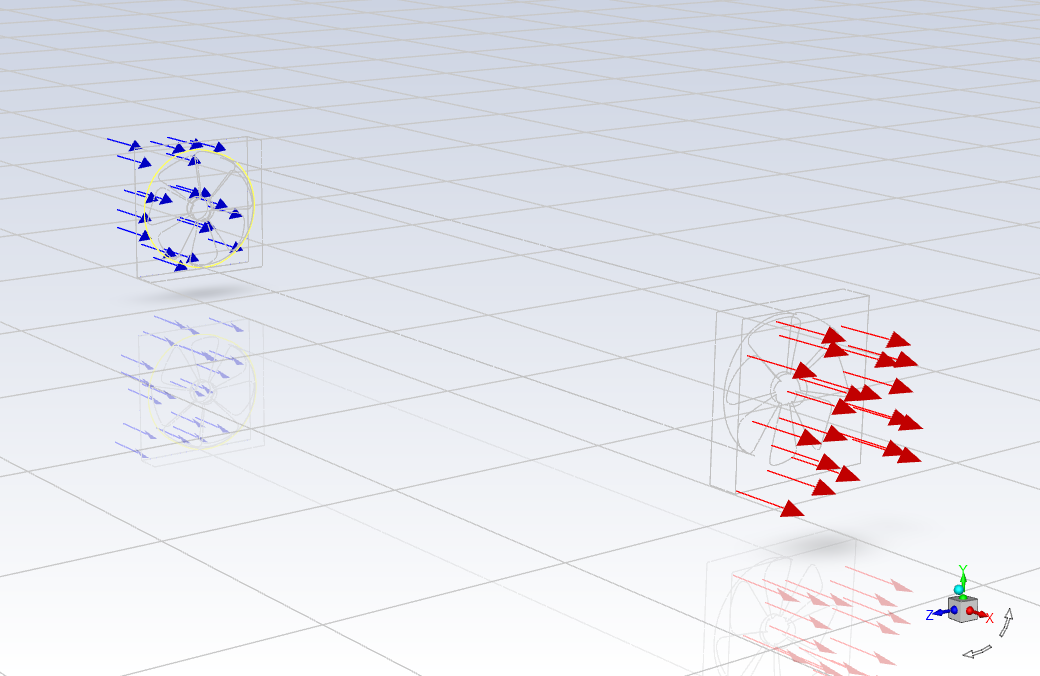
\includegraphics[width=0.7\linewidth]{images/borde.png}
    \caption{Condiciones de borde aplicadas en ANSYS Fluent.}
    \label{fig:borde}
\end{figure}

\subsection{Cálculo y Convergencia}
Se seleccionó un esquema de discretización \textit{semi-implicit} y un método de acoplamiento presión-velocidad (SIMPLE o SIMPLER), ajustando el número de iteraciones hasta alcanzar convergencia (generalmente cuando los residuos de velocidad, presión y turbulencia descendieron a un valor menor a $10^{-4}$). El cálculo se realizó en iteraciones sucesivas, monitoreando parámetros de interés como la velocidad promedio en la sección de salida y la presión en la región del ventilador.



\subsection{Obtención de Resultados}
Tras la convergencia, se post-procesaron los resultados para extraer.
\begin{itemize}
    \item \textbf{Distribución de velocidades:} Campos vectoriales y escalas de magnitud de velocidad en el interior del túnel.
    \item \textbf{Presiones estática y dinámica:} Perfiles a lo largo de la sección principal, útiles para determinar pérdidas de carga.
    \item \textbf{Líneas de corriente (streamlines):} Visualización del patrón de flujo e identificación de zonas de recirculación.
    \item \textbf{Distribución de temperatura (opcional):} En caso de habilitar transferencia de calor para comparar con datos de la cámara térmica.
\end{itemize}

\section{Validación del Modelo CFD mediante Comparación de Datos}
\subsection{Diseño de las Pruebas de Validación}
Para validar el modelo numérico se definieron ensayos experimentales con el túnel de viento a distintas velocidades del ventilador (en un rango de 833-4200 RPM). Durante cada ensayo:
\begin{itemize}
    \item Se midió el consumo de corriente y voltaje del motor para relacionarlo con la potencia.
    \item Se registró la velocidad del flujo de aire en varios puntos de la cámara principal mediante el sensor de flujo calibrado.
    \item Se monitorearon vibraciones y temperaturas, en busca de correlaciones con las distribuciones de velocidad simuladas.
\end{itemize}

\subsection{Comparación Cualitativa y Cuantitativa}
\begin{enumerate}
    \item \textbf{Comparación cualitativa:} Se inspeccionaron visualmente las líneas de flujo y zonas de recirculación detectadas en la simulación, contrastándolas con el comportamiento real observado (por ejemplo, con humo trazador o patrones de polvo muy ligero en el túnel).
    \item \textbf{Comparación cuantitativa:} Se emplearon estadísticos como el \textit{error porcentual medio} (MAPE) o la diferencia absoluta promedio entre las velocidades simuladas y las medidas por el anemómetro. 

    \begin{equation}
    \text{Error\%} = \frac{\lvert v_{\text{sim}} - v_{\text{exp}} \rvert}{v_{\text{exp}}} \times 100
    \end{equation}

    Se establecieron límites de aceptación basados en la precisión de los sensores y la complejidad del fenómeno (un error menor al 10\% se consideró razonable para este tipo de prototipo).
\end{enumerate}

\subsection{Ajustes y Retroalimentación}
En caso de observar discrepancias mayores a las esperadas, se realizaron ajustes en el modelo CFD:
\begin{itemize}
    \item Refinar la malla en zonas críticas y aumentar el número de capas en la región de la capa límite.
    \item Modificar el modelo de turbulencia o los valores de parámetros en \texttt{k-$\epsilon$}.
    \item Incluir efectos de compresibilidad o calor, si fuera necesario.
\end{itemize}

Tras cada ajuste, se repitió el proceso de simulación y validación, iterando hasta lograr un nivel satisfactorio de concordancia entre datos experimentales y simulados.

%%%%%%%%%%%%%%%%%%%%%%%%%%%%%%%%%%%%%%%%%%%%%%%%%%%%%%%%%%%%%%%
\section{Evaluación Cualitativa de los Datos}

Este apartado se centra exclusivamente en la revisión y análisis cualitativo de los datos disponibles, con el propósito de determinar si, en un futuro, podrían emplearse para entrenar un modelo de mantenimiento predictivo. A continuación, se describe la metodología básica para dicha evaluación.

\subsection{Recopilación y Organización de Datos}
En primer lugar, se reúnen y clasifican los datos provenientes de:
\begin{enumerate}
    \item \textbf{Prototipo Experimental:} Incluye mediciones de RPM, velocidad del viento, vibraciones y temperaturas, así como parámetros eléctricos (corriente y voltaje).
    \item \textbf{Simulación CFD:} Ofrece distribuciones de velocidad, gradientes de presión y patrones de flujo bajo diferentes regímenes de rotación del ventilador.
\end{enumerate}
La información se integra en un único repositorio o formato que permita su revisión conjunta (tablas de datos, hojas de cálculo, etc.).

\subsection{Análisis Exploratorio}
Tras la unificación de los datos, se realiza un examen cualitativo con el fin de:
\begin{itemize}
    \item \textbf{Visualizar Tendencias:} Inspeccionar, mediante gráficas o listados, cómo varían las RPM o la velocidad del viento en distintos escenarios de operación o configuraciones de la simulación.
    \item \textbf{Comparar Fuentes de Datos:} Identificar posibles divergencias entre las lecturas experimentales y los resultados simulados para detectar comportamientos atípicos o inconsistencias.
    \item \textbf{Relaciones Básicas:} Explorar, de manera cualitativa, si un incremento en las RPM coincide con mayores vibraciones o si cambios en la velocidad del viento repercuten de forma notoria en la corriente consumida.
\end{itemize}

\subsection{Formulación de Observaciones Cualitativas}
Con base en las tendencias y comparaciones realizadas, se elaboran conclusiones preliminares que describen de forma no cuantificada:
\begin{itemize}
    \item \textbf{Patrones de Operación:} Zonas de funcionamiento estable versus rangos en los que se observan irregularidades como altos picos de vibración o sobrecalentamiento.
    \item \textbf{Semejanzas y Discrepancias:} Grado de concordancia entre los valores medidos y las predicciones de la simulación, indicando si ésta refleja adecuadamente la realidad o si existen supuestos simplificados.
    \item \textbf{Indicadores de Posible Falla:} Apreciaciones sobre signos potenciales de desgaste en el ventilador (p.ej., aumento sostenido de temperatura o vibraciones no esperadas).
\end{itemize}

\subsection{Conclusión y Viabilidad para un Futuro Modelo}
Finalmente, se emite un juicio cualitativo acerca de si los datos recabados presentan la variedad y consistencia necesarias para, en el futuro, generar un modelo de mantenimiento predictivo. En caso afirmativo, se sugiere profundizar en análisis estadísticos o incluir más variables de interés. Si no se detecta información suficiente, se recomienda ampliar la toma de datos o refinar la metodología de medición y simulación.

\noindent
Este proceso de evaluación cualitativa constituye un punto de partida para determinar de manera inicial la factibilidad de desarrollar herramientas predictivas a partir de los datos de RPM, velocidad de viento y demás variables monitorizadas tanto en la prueba experimental como en la simulación.


%%%%%%%%%%%%%%%%%%%%%%%%%%%%%%%%%%%%%%%%%%%%%%%%%%%%%%%%%%%%%%%%
\section{Flujo de Trabajo}
En términos generales, el flujo de trabajo para realizar una prueba experimental y su validación CFD es:
\begin{enumerate}
    \item \textbf{Configuración de la prueba:} El usuario accede a la interfaz web y ajusta la velocidad del ventilador y la lista de sensores a monitorear.
    \item \textbf{Adquisición de datos:} La interfaz web envía la configuración a la API y el Arduino comienza a leer los sensores, transmitiendo datos que se almacenan en SQLite.
    \item \textbf{Generación del modelo CFD:} Se prepara la geometría y la malla en ANSYS, aplicando condiciones de contorno que emulen las condiciones del prototipo (velocidad, caudal, presión, etc.).
    \item \textbf{Ejecución de la simulación:} Se corre el solver CFD y se monitorean los residuos hasta alcanzar la convergencia.
    \item \textbf{Post-procesado y extracción de datos:} Se obtienen campos de velocidad, presión, temperatura, etc. 
    \item \textbf{Comparación y validación:} Se contrasta la información simulada con las mediciones experimentales de velocidad, corriente, vibración y temperatura.
    \item \textbf{Ajuste o refinamiento:} Se corrige la malla o se varían los parámetros del modelo CFD para reducir diferencias con la realidad.
    \item \textbf{Evaluación cualitativa de datos:} Se analizan las fuentes y calidad de datos para evaluar el desarrollo de modelos de mantenimiento predictivos basados en machine learning.
\end{enumerate}

\pagebreak
\section{Resumen de la Metodología}
La metodología propuesta integra el diseño de un prototipo físico de túnel de viento a escala con un sistema automatizado de adquisición de datos que comunica los sensores con una API REST y una interfaz web interactiva. El almacenamiento en \texttt{SQLite} permite un acceso rápido y versátil a las mediciones, facilitando la comparación entre datos experimentales y simulaciones CFD en ANSYS. La validación se establece al correlacionar los valores de velocidad, temperatura y vibración medidos con los campos numéricos simulados, permitiendo ajustar el modelo computacional hasta lograr concordancias aceptables. Esta arquitectura modular es escalable y puede adaptarse para futuras extensiones, como la incorporación de algoritmos de machine learning o la migración a sistemas de mayor complejidad en escenarios mineros reales.
